% !TeX root = ../main.tex

\begin{frame}
  \frametitle{{\small The Topological Coverage Criterion (TCC)}}

  \begin{textblock*}{12cm}(1cm,2cm)
    \begin{small}
      Bounded domain $D$ with boundary $B$.\vspace{1ex}

      \only<2-4>{Geometric sample of $D$.\vspace{1ex}}

      \only<3,4>{Use homology to identify holes in coverage.}
    \end{small}
  \end{textblock*}

  \begin{textblock*}{12cm}(1cm,5cm)
    \includegraphics<1>[trim=200 600 200 800, clip, width=0.5\textwidth]{figures/nocover/surf}
    \includegraphics<2>[trim=200 600 200 800, clip, width=0.5\textwidth]{figures/nocover/samples}
    % \includegraphics<2>[trim=200 600 200 800, clip, width=0.5\textwidth]{figures/nocover/cover}
    \includegraphics<3>[trim=200 600 200 800, clip, width=0.5\textwidth]{figures/nocover/complex}
    \includegraphics<4>[trim=200 600 200 800, clip, width=0.5\textwidth]{figures/cover/complex}
  \end{textblock*}
\end{frame}

\begin{frame}
  \frametitle{{\small TCC $\to$ SFA}}

  \begin{textblock*}{12cm}(1cm,2cm)
    \only<1,2>{Consider partial coverage.\vspace{1ex}}

    \only<2>{Suppose points sample $f : D\to \R$.}
    \only<3>{Define our boundary as a sublevel set $B_\omega$ of $f$.}
    \only<4>{Determine coverage of $D\setminus B_\omega$.}
  \end{textblock*}

  \begin{textblock*}{12cm}(1cm,5cm)
    \includegraphics<1>[trim=200 600 200 800, clip, width=0.5\textwidth]{figures/partial/complex}
    \includegraphics<2>[trim=200 600 200 800, clip, width=0.5\textwidth]{figures/partial1/samples}
    \includegraphics<3>[trim=200 600 200 800, clip, width=0.5\textwidth]{figures/partial2/samples}
    \includegraphics<4>[trim=200 600 200 800, clip, width=0.5\textwidth]{figures/partial2/complex}
    % \includegraphics<3>[trim=200 600 200 800, clip, width=0.5\textwidth]{figures/nocover/cover}
    % \includegraphics<4>[trim=200 600 200 800, clip, width=0.5\textwidth]{figures/nocover/complex}
    % \includegraphics<5>[trim=200 600 200 800, clip, width=0.5\textwidth]{figures/cover/complex}
  \end{textblock*}
\end{frame}

\begin{frame}
  \frametitle{{\small {\color{red} \textbf{Goal:}} Analyze $f$ where we have confirmed coverage.}}

  \begin{textblock*}{12cm}(1cm,2cm)
    \begin{enumerate}
      \item<2,3> Check for coverage of $D\setminus B_\omega$,
      \item<3> Analyze $f$ in $D\setminus B_\omega$.
    \end{enumerate}
  \end{textblock*}

  \begin{textblock*}{12cm}(1cm,5cm)
    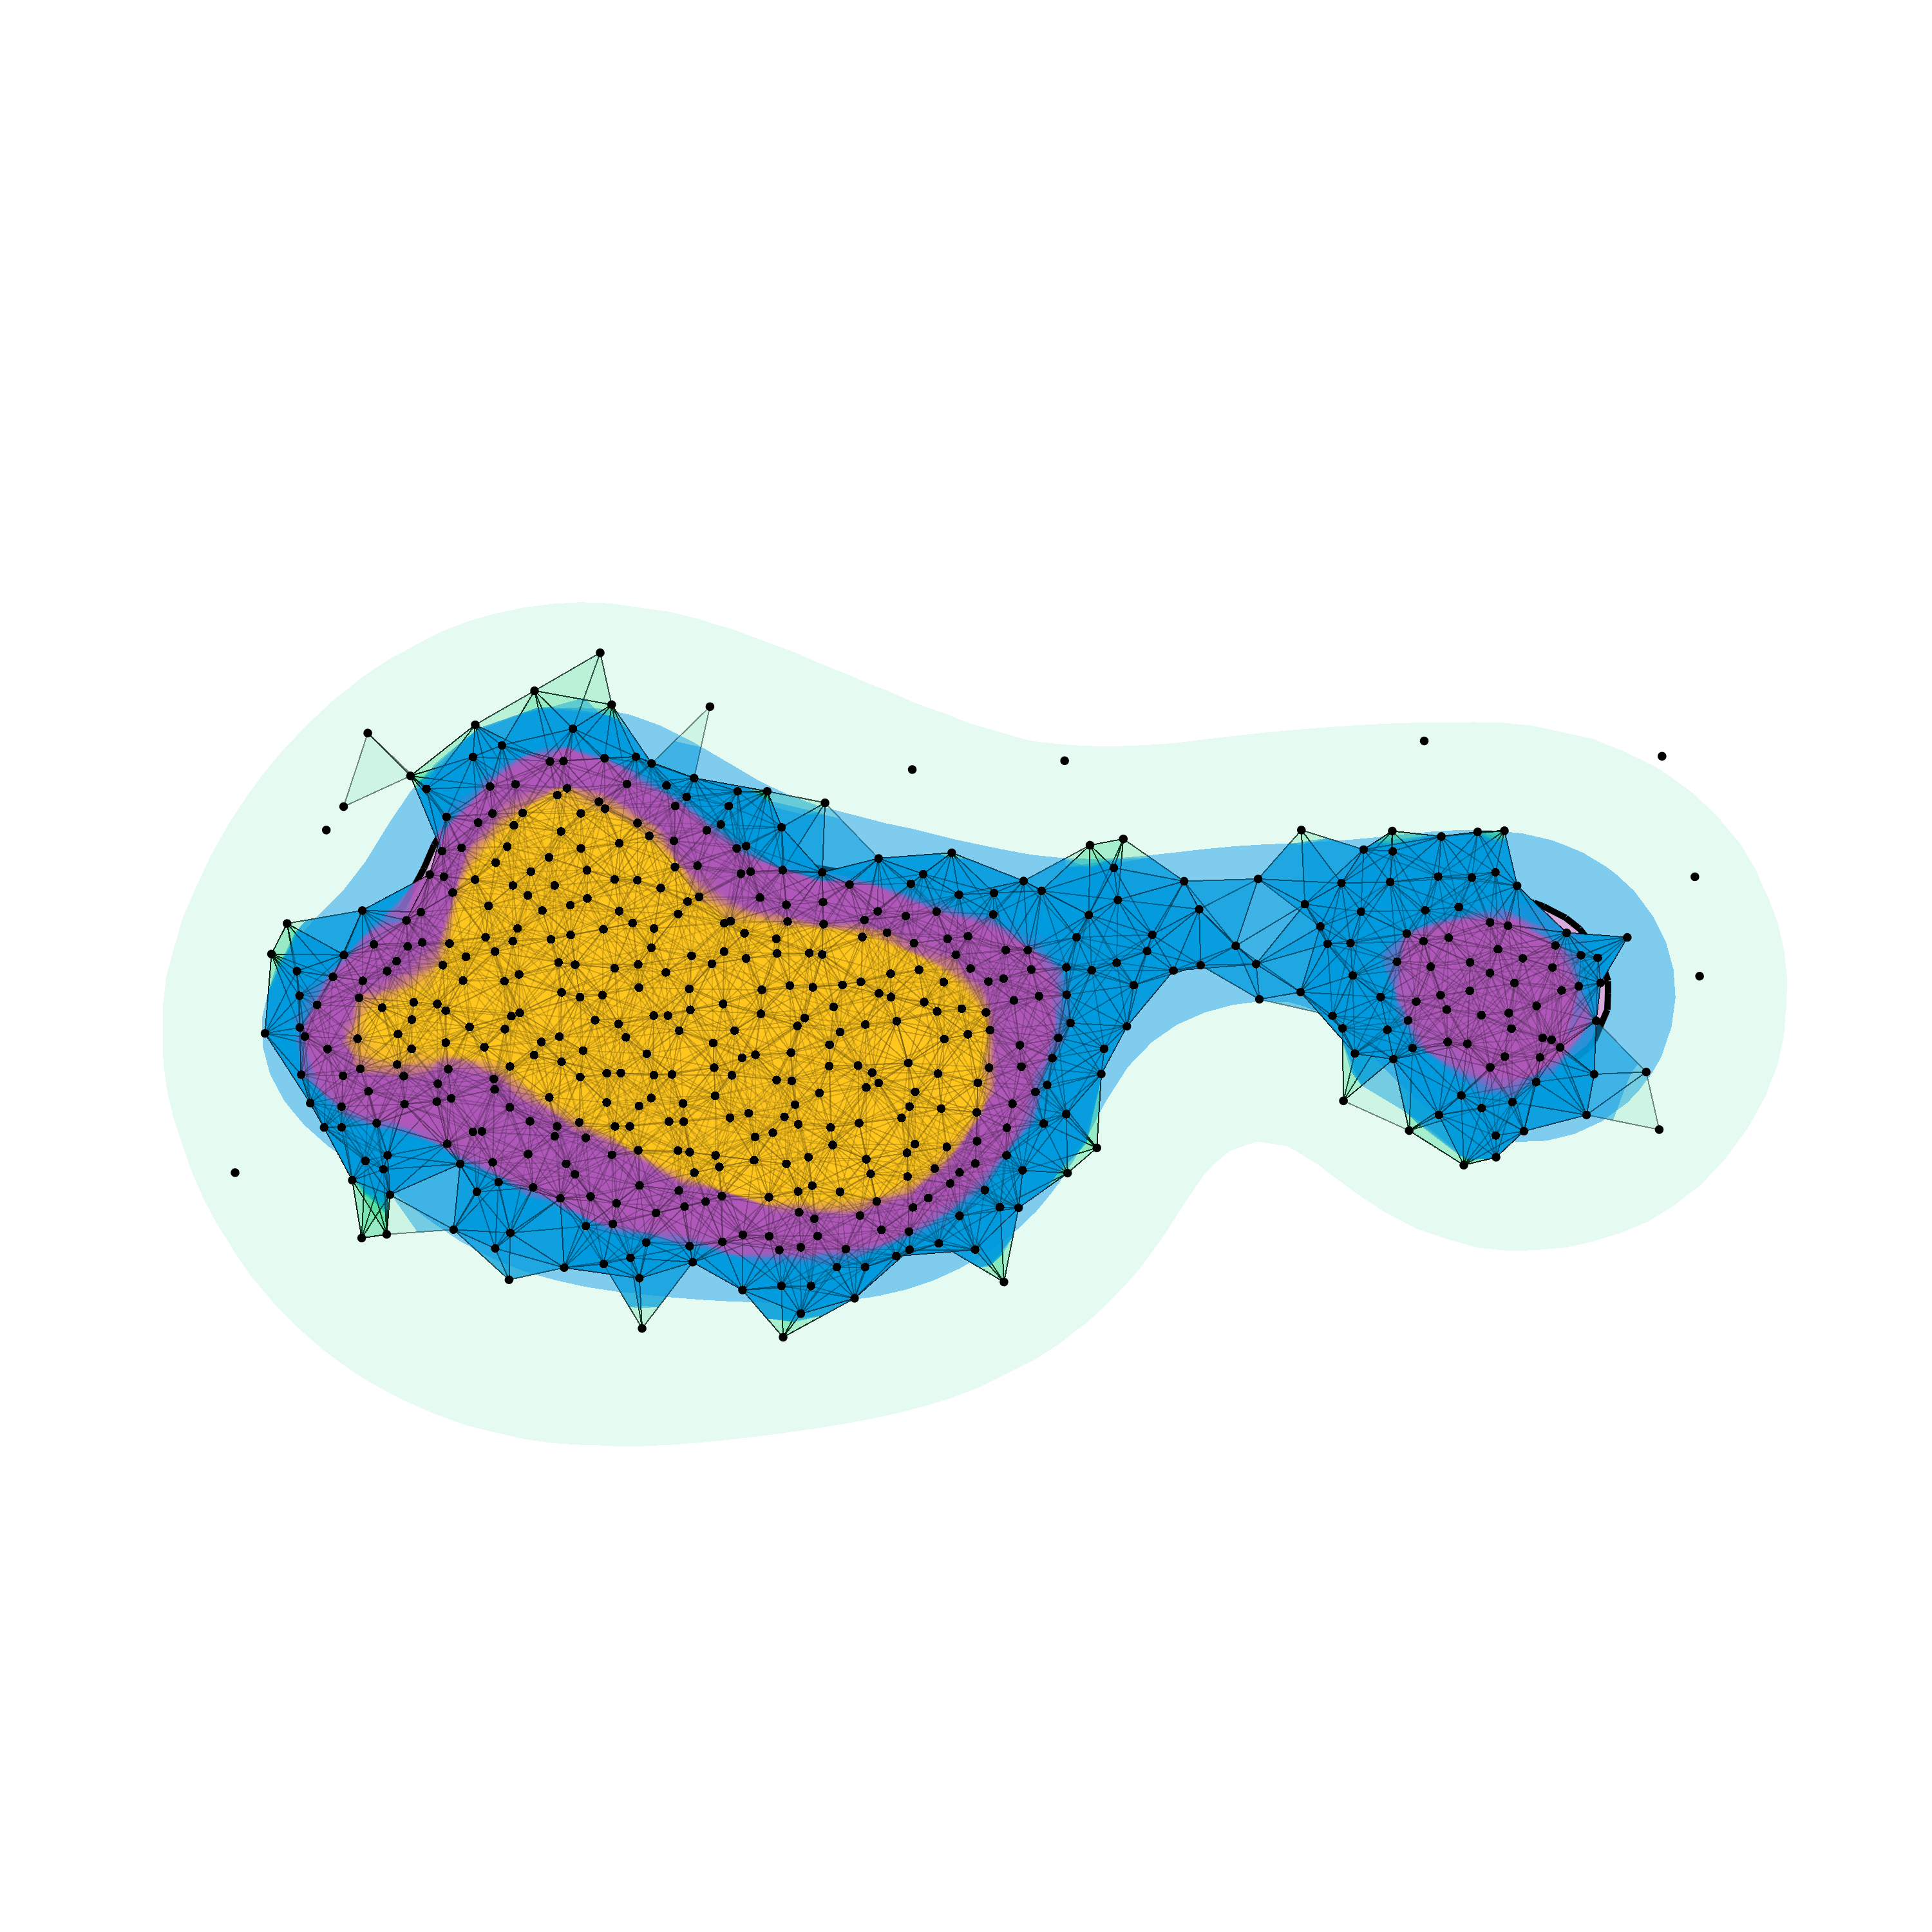
\includegraphics[trim=200 600 200 800, clip, width=0.5\textwidth]{figures/samples/scalar1}
  \end{textblock*}
\end{frame}
